\documentclass[a4paper, 11pt]{article}
\usepackage[utf8x]{inputenc}
\usepackage[IL2]{fontenc}
\usepackage[czech]{babel}
\usepackage{times}

\usepackage{url}
\usepackage[unicode]{hyperref}
\usepackage[hyphenbreaks]{breakurl}

\usepackage{scrextend}
\usepackage{graphicx}
\usepackage[left=2cm,text={17cm, 24cm},top=3cm]{geometry}
\urlstyle{rm}
\date{}
\begin{document}
\pagenumbering{gobble}
\begin{center}
    \Huge
    \textsc{Vysoké učení technické v Brně\\\huge Fakulta informačních technologií}\\
    \vspace{\stretch{0.382}}
    \LARGE
    Typografie a publikování – 4. projekt\\\Huge 
    Bibliografické citace
    \vspace{\stretch{0.618}}
\end{center}
{\Large \today \hfill Vadim Goncearenco}
\newpage
\pagenumbering{arabic}

\section{Egyptské písmo a egyptienka}
\subsection{Definice}
Egyptské hieroglyfické písmo nebo hieroglyfy, je jedním ze systémů egyptského písma. Používalo se v Egyptě téměř 3500 let, počínaje přelomem 4. a 3. tisíciletí před naším letopočtem. Jde o obrázkové písmo doplněné o hláskové znaky, to znamená, že kombinuje prvky ideografického, slabičného a fonetického písma. Podrobnější definici se dá přečíst na stránce Wikipedii \cite{wiki_en}. 
\subsection{Historie a původ hieroglyfů}
Jak je uvedeno v \cite{worldhistory}, původ egyptských hieroglyfů je špatně pochopen. Existuje však několik hypotéz, které byly vysloveny. Jeden z nejpřesvědčivějších názorů tvrdí, že pocházejí ze skalních obrázků vytvořených pravěkými loveckými komunitami. Uvedené komunity pravděpodobně žili v poušti západně od Nilu a zjevně znaly koncept komunikace pomocí vizuálních představ.

Podle všeho egypťané měli dva zvláštní druhy písma: první, nazývaný obyčejný,
naučil se každý. Ten druhý ale, zvaný posvátný, byl známý pouze kněžím a předával se od otce k synovi mezi tajnými věcmi. (viz. \cite{between_pride_and_prejudice})
\subsection{Dešifrování egyptského písma}
Z \cite{tabula} je zřejmé, že všechny středověké a raně novověké pokusy o dešifrování byly brzděny základním předpokladem, že hieroglyfy zaznamenávaly myšlenky a nikoli zvuky jazyka. Protože nebyly k dispozici žádné dvojjazyčné texty, mohl být jakýkoli takový symbolický „překlad“ navržen bez možnosti ověření.

Jak uvádí James Allen ve svém dílu \cite{middle_egyptian}, teprve díky Athanasiu Kircherovi v první polovině 17. století začali učenci uvažovat o tom, že hieroglyfy mohou také představovat zvuky.

Průlom v dešifrování nastal až s objevem Rosettské desky Napoleonovými vojsky v roce 1799. Úplné rozluštění nakonec provedl Jean-François Champollion ve 20. letech 19. století. (viz. \cite{egypt_today})
\subsection{Egyptienka}
Egyptienka, nebo angl. ``slab serif'' (nazývané také mechanické, čtvercové serifové, starožitné nebo egyptské) písmo, je typ patkového písma charakterizovaného tlustými, blokovitými patkami. Typ ``slab serif'' byl poprvé představen londýnským typografem Vincentem Figginsem pod názvem „Antique“, který se objevil v typovém exempláři datovaném rokem 1815. (viz. \cite{slab_serif_england}\cite{iveta_dvokov})
\begin{figure}[htb]
\centering
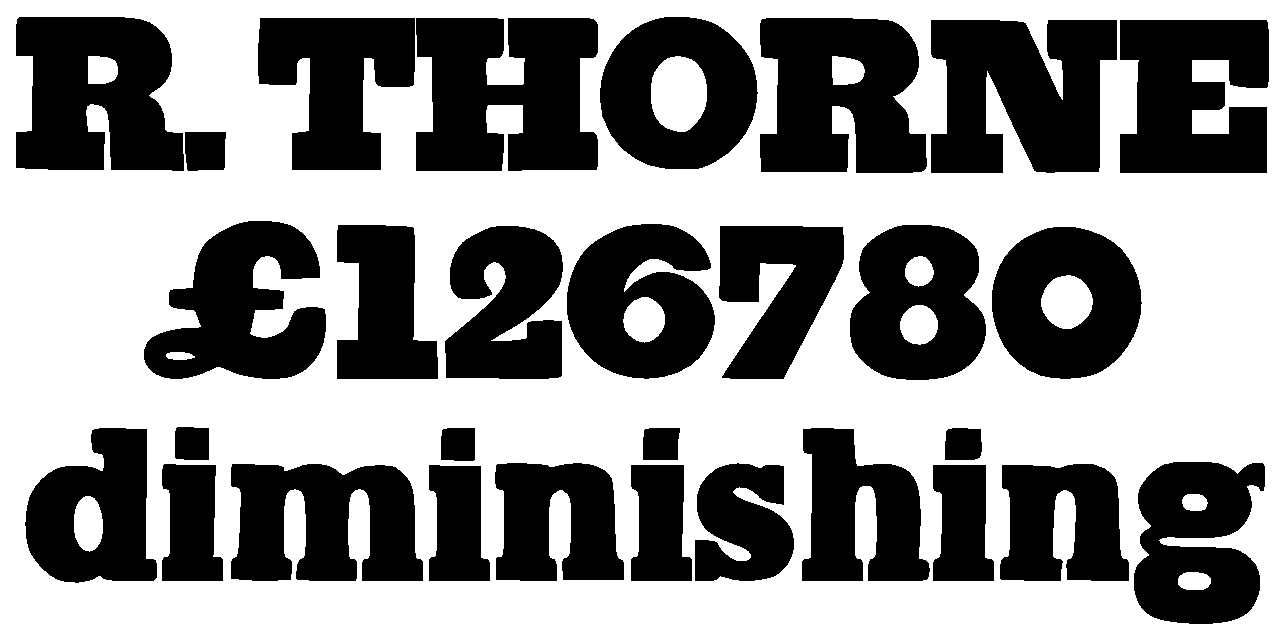
\includegraphics[scale=0.3]{slab_serif.eps}
\caption{Příklad egiptienky z monografie roku 1921. \cite{keith_tam}}
\end{figure}

Ale teprve po Napoleonově egyptském tažení a šíření obrázků a popisů egyptských hieroglyfů se stala egiptienka skutečně populární.

Kvůli jasné a výrazné povaze velkých patek se vzory s některými charakteristikami slabých patek egiptienka se také často používala pro drobný tisk, například při tisku na psacích strojích a na novinový papír.

Jak výstižně zdůraznil Aanya Kumar ve svém časopise \cite{aanya_kumar}, historie egyptienky byla také nerozlučně spjata s nástupem průmyslové revoluce a stala se vlastně jedním z jejích nejvýmluvnějších symbolů.
\newpage
\bibliographystyle{czechiso}
\renewcommand{\refname}{Literatura}
\bibliography{proj4}
\end{document}
